% !TeX program = xelatex
\documentclass[11pt,a4paper]{article}

\usepackage{fontspec}
\usepackage[table]{xcolor}
\usepackage{graphicx}
\usepackage{tabularx}
\usepackage{longtable}
\usepackage{array}
\usepackage{hyperref}
\usepackage{tikz}
\usepackage{fancyhdr}
\usepackage{caption}
\usepackage{float}
\usepackage{needspace}
\usepackage{enumitem}
\usepackage[section]{placeins}
\usetikzlibrary{trees,positioning,calc,shapes.geometric}

\setmainfont[AutoFakeSlant=0.2]{Microsoft YaHei}
\setsansfont{Microsoft YaHei}
\newfontfamily\covertitlefont[AutoFakeBold=2]{STZhongsong}
\newfontfamily\coverinfofont{Microsoft YaHei}
\XeTeXlinebreaklocale "zh"
\XeTeXlinebreakskip=0pt plus 1pt
\renewcommand{\contentsname}{目录}
\renewcommand{\figurename}{图}
\renewcommand{\tablename}{表}
\setlength{\oddsidemargin}{-0.15in}
\setlength{\evensidemargin}{-0.15in}
\setlength{\textwidth}{6.5in}
\setlength{\topmargin}{-0.55in}
\setlength{\textheight}{9.65in}

\definecolor{Forest}{HTML}{173F35}
\definecolor{Pine}{HTML}{2F6657}
\definecolor{Sage}{HTML}{BFD8CB}
\definecolor{Clay}{HTML}{C86448}
\definecolor{Sand}{HTML}{F2E8D5}
\definecolor{Ink}{HTML}{202725}
\definecolor{Mist}{HTML}{F3F6F4}
\definecolor{LineGray}{HTML}{C9D2CE}
\definecolor{PaleCover}{HTML}{EAF4EE}
\definecolor{Leaf}{HTML}{4D806E}
\definecolor{CSUBlue}{HTML}{2F6657}
\definecolor{CSUDark}{HTML}{173F35}
\definecolor{CSUPale}{HTML}{EAF4EE}
\definecolor{CSUSoft}{HTML}{F3F6F4}
\definecolor{CSUGold}{HTML}{7EA996}

\hypersetup{
  colorlinks=true,
  linkcolor=Forest,
  urlcolor=Clay,
  citecolor=Forest,
  pdftitle={BSR滑雪装备租赁与维护管理系统：需求设计文档},
  pdfauthor={汪子涵}
}

\setlength{\parindent}{2em}
\setlength{\parskip}{0.28em}
\renewcommand{\arraystretch}{1.28}
\linespread{1.13}\selectfont
\setlength{\tabcolsep}{3.4pt}
\setlength{\emergencystretch}{1.5em}
\setlength{\parskip}{0.28em}
\renewcommand{\topfraction}{0.92}
\renewcommand{\bottomfraction}{0.85}
\renewcommand{\textfraction}{0.07}
\renewcommand{\floatpagefraction}{0.82}
\setcounter{topnumber}{3}
\setcounter{bottomnumber}{2}
\setcounter{totalnumber}{4}
\raggedbottom
\setlength{\LTpre}{0.5em}
\setlength{\LTpost}{0.5em}
\newcommand{\toprule}{\hline}
\newcommand{\midrule}{\hline}
\newcommand{\bottomrule}{\hline}
\makeatletter
\renewcommand\section{\@startsection{section}{1}{0pt}{-3.0ex plus -1ex minus -.2ex}{1.6ex plus .2ex}{\LARGE\bfseries\color{Forest}}}
\renewcommand\subsection{\@startsection{subsection}{2}{0pt}{-2.6ex plus -1ex minus -.2ex}{1.2ex plus .2ex}{\Large\bfseries\color{Forest}}}
\renewcommand\subsubsection{\@startsection{subsubsection}{3}{0pt}{-2.2ex plus -1ex minus -.2ex}{0.9ex plus .2ex}{\large\bfseries\color{Pine}}}
\renewcommand\paragraph{\@startsection{paragraph}{4}{0pt}{-1.9ex plus -.8ex minus -.2ex}{0.7ex plus .2ex}{\normalsize\bfseries\color{Pine}}}
\let\@afterindentfalse\@afterindenttrue
\makeatother
\setcounter{secnumdepth}{4}
\setcounter{tocdepth}{3}
\pagestyle{fancy}
\setlength{\headheight}{13pt}
\fancyhf{}
\lhead{\small\color{Leaf} BSR 滑雪装备租赁与维护管理系统}
\rhead{\small\color{Leaf}\nouppercase{\leftmark}}
\cfoot{\small\color{Leaf}第{\thepage}页}
\renewcommand{\headrulewidth}{0.45pt}
\renewcommand{\footrulewidth}{0pt}
\captionsetup{font=small,labelfont={bf,color=CSUDark},textfont={color=Ink},labelsep=quad,skip=9pt}

\newcolumntype{Y}{>{\raggedright\arraybackslash}X}
\newcolumntype{L}[1]{>{\raggedright\arraybackslash}p{#1}}
\newcommand{\tablehead}[1]{\bfseries #1}
\newcommand{\source}[2]{\href{#1}{#2}}
\newcommand{\portraitdiagram}[3]{%
  \par\vspace{0.55cm}\noindent
  \begin{minipage}{\textwidth}\centering
  \includegraphics[width=\textwidth,height=0.68\textheight,keepaspectratio]{#1}
  \captionof{figure}{#2}\label{#3}
  \end{minipage}\par\vspace{0.75cm}}
\newcommand{\fixeddiagram}[3]{%
  \par\medskip\noindent
  \begin{minipage}{\textwidth}\centering
  \includegraphics[width=\textwidth,height=0.62\textheight,keepaspectratio]{#1}
  \captionof{figure}{#2}\label{#3}
  \end{minipage}\par\medskip}
\newcommand{\singlepagediagram}[3]{%
  \par\vspace*{\fill}\noindent
  \begin{minipage}{\textwidth}\centering
  \includegraphics[width=\textwidth,height=0.67\textheight,keepaspectratio]{#1}
  \captionof{figure}{#2}\label{#3}
  \end{minipage}\par\vspace*{\fill}\null\clearpage}
\newcommand{\tallsequence}[3]{%
  \par\vspace*{\fill}\noindent
  \begin{minipage}{\textwidth}\centering
  \includegraphics[width=\textwidth,height=0.88\textheight,keepaspectratio]{#1}
  \captionof{figure}{#2}\label{#3}
  \end{minipage}\par\vspace*{\fill}\null\clearpage}
\newcommand{\businessdiagram}[3]{%
  \par\vspace{0.12cm}\noindent
  \begin{minipage}{\textwidth}\centering
  \includegraphics[width=0.80\textwidth,height=0.40\textheight,keepaspectratio]{#1}
  \captionof{figure}{#2}\label{#3}
  \end{minipage}\par\vspace{0.18cm}}
\newcommand{\businessdiagramcompact}[3]{%
  \par\noindent
  \begin{minipage}{\textwidth}\centering
  \includegraphics[width=0.66\textwidth,height=0.32\textheight,keepaspectratio]{#1}
  \captionof{figure}{#2}\label{#3}
  \end{minipage}\par}
\newcommand{\dbtable}[3]{%
  \par\medskip\noindent
  \begin{minipage}{\textwidth}
  \centering
  {\footnotesize
  \captionof{table}{#1}\label{#2}\par\vspace{0.05em}
  \begin{tabular}{L{4.0cm}L{3.1cm}L{2.6cm}L{4.9cm}}
  \toprule
  \tablehead{字段名称} & \tablehead{中文描述} & \tablehead{数据类型} & \tablehead{约束条件}\\
  \midrule
  #3
  \bottomrule
  \end{tabular}}
  \end{minipage}\par\medskip}

\begin{document}
\begin{titlepage}
\thispagestyle{empty}
\vspace*{1.55cm}
\noindent
\begin{minipage}[c]{0.76\textwidth}
  \noindent{\coverinfofont\color{Leaf}\fontsize{15.5}{22}\selectfont 系统分析与设计课程大作业}
\end{minipage}
\hfill
\begin{minipage}[c]{0.18\textwidth}
  \raggedleft
\includegraphics[width=1.65cm]{csu-logo-official.png}
\end{minipage}

\vspace{0.35cm}
\noindent{\color{Leaf}\rule{\textwidth}{0.65pt}\par}

\vspace{2.05cm}
\noindent{\coverinfofont\color{CSUDark}\fontsize{29}{41}\selectfont\bfseries
BSR 滑雪装备租赁与\par
维护管理系统\par}

\vspace{0.55cm}
\noindent{\coverinfofont\color{Clay}\fontsize{16}{24}\selectfont\bfseries
业务建模 · 需求 · 分析 · 设计\par}

\vfill
\hfill
\begin{minipage}{7.25cm}
{\coverinfofont\color{Leaf}\fontsize{10.5}{16}\selectfont DOCUMENT INFORMATION\par}
\vspace{0.42cm}
\renewcommand{\arraystretch}{1.55}
{\coverinfofont\fontsize{11.5}{18}\selectfont
\begin{tabular}{>{\color{Leaf}}l@{\hspace{0.70cm}}>{\color{CSUDark}\bfseries}l}
课程 & 系统分析与设计 \\
姓名 & 汪子涵 \\
学号 & 1602240223 \\
班级 & 信管2402 \\
\end{tabular}}
\end{minipage}

\vspace{1.15cm}
\noindent{\color{CSUDark}\rule{3.0cm}{2.2pt}}\hspace{0.32cm}{\color{Clay}\rule{0.95cm}{2.2pt}}
\vspace{0.45cm}
\end{titlepage}

\pagenumbering{Roman}
\begingroup
\cfoot{}
\tableofcontents
\clearpage
\endgroup
\pagenumbering{arabic}

\section{业务建模}

\subsection{愿景}

从目标组织代表的视角，说明引入目标系统后最需要改善的一项组织指标。

{\noindent\begin{tabularx}{\textwidth}{L{2.6cm}Y}
\toprule
\bfseries 项目 & \bfseries 内容\\
\midrule
系统 & BSR 滑雪装备租赁与维护管理系统\\
目标组织 & BSR 滑雪租赁公司\\
老大 & Ole Fjordal（BSR 老板）\\
目标 & 缩短顾客从开始办理到领取合适、安全且价格明确的装备所需时间\\
度量指标 & 雪季高峰期 Σ（装备交付时间－开始办理时间）÷ 完成租赁合同数\\
\bottomrule
\end{tabularx}}

\subsubsection*{业务情境}
BSR 经营两家滑雪装备租赁门店。旺季办理租赁时，员工既要确认顾客的尺码与技能水平，也要判断装备是否已经预订、正在出租、处于检查状态或送往维修。若两家门店分别使用纸张和表格记录，同一件装备可能被重复承诺，跨店归还后的实际位置也难以及时同步。

本项目希望建立一套能够支撑门店协同的工作机制。信息系统应当让订单、单件装备、门店位置和维修状态围绕同一条业务记录流转，从而减少电话核对和重复登记。

\subsubsection*{愿景陈述}
面向需要协调租赁、归还与维修工作的 BSR 门店员工和经理，本系统提供一套可远程访问的多门店协同平台。平台以单件装备为追踪单位，使员工能够一次录入顾客需求、即时确认可用装备，并在取件、换装、跨店归还和维修过程中持续更新状态。与分散纸张和独立表格相比，系统提供统一库存视图、冲突校验和审计记录，让顾客更快完成办理，让管理者获得可信的运营信息。

\subsubsection*{范围判断}
本阶段纳入顾客资料、装备查询与推荐、提前预订与合同收费、实际到店与取件、换装、跨店归还、维修工单、经营待办和审计记录；短信通知、会计核算与生产级身份平台不在本阶段范围内。

\clearpage
\subsection{业务用例图}

\portraitdiagram{latex-assets/A2.pdf}{BSR 业务用例图}{fig:a2}

{\noindent\begin{tabularx}{\textwidth}{L{2.2cm}L{2.6cm}L{4.3cm}L{6.2cm}}
\toprule
\bfseries 业务用例 & \bfseries 业务执行者 & \bfseries 对执行者的价值 & \bfseries 价值不满足时的表现\\
\midrule
租赁合适的滑雪装备 & 顾客 & 在合理等待后拿到合身、安全且价格明确的装备。 & 排队混乱、装备不合身、付费档次与实物不符。\\
换装或跨店归还装备 & 顾客 & 装备不合适或行程改变时能就近处理，不必回原店。 & 电话核对拖沓、跨店归还后装备位置不明。\\
协同处理装备维修 & 维修承包商 & 拿到完整故障信息和明确的交接、验收安排。 & 纸质登记簿传递慢，修好后多久能再出租无人清楚。\\
\bottomrule
\end{tabularx}}

\clearpage
\subsection{业务序列图}

业务用例图中的三项业务分别配置一张现状业务序列图和一张改进业务序列图，使业务边界、现状问题与改进方案逐项对应。

改进的方向可以归为三类：一是把物流变成信息流，减少装备、单据和人员在门店之间的实际移动；二是让信息流自动化，原来靠人记、靠人算、靠人传的环节改由系统直接完成；三是封装领域逻辑，把适配判断、价格计算和可用性校验等专家经验沉淀到系统中，降低对个人经验的依赖。下面每张改进图都按这三类逐条说明。

\subsubsection{租赁合适的滑雪装备}

现状由顾客申请触发：员工依靠 Excel、人工适配与计价和纸质合同办理，排队状态、装备位置与维修状态难以及时共享。参与现状流程的角色划分如下。

\businessdiagramcompact{latex-assets/A3.pdf}{租赁合适的滑雪装备 - 现状业务序列图}{fig:a3-rent-current}

{\noindent\begin{tabularx}{\textwidth}{L{2.4cm}L{3.0cm}L{4.4cm}L{5.5cm}}
\toprule
\bfseries 角色类型 & \bfseries 角色 & \bfseries 现状职责 & \bfseries 改进后是否由系统取代\\
\midrule
业务执行者 & 顾客 & 说明租赁需求与身体参数，确认方案，领取装备。 & 否，仍由顾客参与，但交互量减少。\\
业务工人 & 门店员工 & 查询顾客与库存、人工判断适配与安全、人工计价、填写纸质合同、收款。 & 部分取代：查询、判断、计价与登记转交系统，面对顾客的解释与最终确认保留。\\
业务执行者 & 第三方支付服务 & 处理收费并返回支付结果。 & 否，仍由外部系统承担本阶段不提供的支付业务。\\
业务实体 & Excel 工作簿 & 保存顾客、库存、出租与维修记录。 & 是，转由统一数据库承担。\\
业务实体 & 纸质租赁合同 & 记录合同内容作为双方凭证。 & 是，转由电子合同承担。\\
\bottomrule
\end{tabularx}}



\clearpage
改进流程保持相同的起点与终点，将一次录入、跨店查询、适配与安全校验、价格明细、合同和审计责任交给统一系统。

\businessdiagram{latex-assets/A4.pdf}{租赁合适的滑雪装备 - 改进业务序列图}{fig:a4-rent-improved}

{\noindent\begin{tabularx}{\textwidth}{L{3.0cm}L{4.8cm}L{7.5cm}}
\toprule
\bfseries 改进类别 & \bfseries 改进点 & \bfseries 对应的系统责任\\
\midrule
\mbox{物流变信息流} & 纸质合同改为在线的电子合同，并与审计记录同步；顾客不必在门店间往返确认库存。 & 合同、装备状态和支付结果在同一条业务记录上流转，门店员工在线查看即可。\\
\mbox{信息流自动化} & 顾客资料与预约信息一次录入后跨环节复用；排队顺序、当前环节和开始办理时间由系统自动记录。 & 办理任务自动建立与更新，避免重复登记和重复询问。\\
\mbox{信息流自动化} & 两店库存、租期冲突、维修状态与安全检查有效期由系统统一校验。 & 候选装备查询与筛选自动完成，不再依赖电话核对。\\
\mbox{封装领域逻辑} & 适配建议、推荐顺序与推荐理由由系统按尺码、技能等级和偏好生成。 & 适配知识和拒绝规则沉淀为系统规则，新员工也能给出一致的推荐。\\
\mbox{封装领域逻辑} & 租金、档次差价和费用明细由系统按统一价目计算并在付款前展示。 & 价格计算集中在系统内，避免人工计价造成的口径不一致。\\
\bottomrule
\end{tabularx}}

\clearpage
\subsubsection{换装或跨店归还装备}

现状依靠纸质合同、分散的 Excel 记录和电话核对原门店信息，装备检查、费用调整和位置变更均需人工完成。这里最典型的是异店归还：受理门店看不到原门店当天更新的记录，只能打电话确认。

\businessdiagram{latex-assets/A3_02.pdf}{换装或跨店归还装备 - 现状业务序列图}{fig:a3-return-current}

{\noindent\begin{tabularx}{\textwidth}{L{2.4cm}L{3.0cm}L{4.4cm}L{5.5cm}}
\toprule
\bfseries 角色类型 & \bfseries 角色 & \bfseries 现状职责 & \bfseries 改进后是否由系统取代\\
\midrule
业务执行者 & 顾客 & 提出换装或跨店归还申请，交回装备，领取替换装备或归还凭证。 & 否，仍由顾客参与。\\
业务工人 & 受理门店员工 & 查找纸质合同、检查装备、人工计算差价与损坏费用、手工登记结果。 & 部分取代：查询、计价与登记转交系统，实物检查和顾客沟通保留。\\
业务工人 & 原门店员工 & 通过电话提供合同、装备位置和出租状态。 & 是，该核对环节取消，改由系统直接给出跨店数据。\\
业务执行者 & 第三方支付服务 & 处理补款或退款。 & 否，仍由外部系统承担。\\
业务实体 & 纸质租赁合同 & 保存合同与租期，作为现场登记载体。 & 是，转由电子合同承担。\\
业务实体 & Excel 工作簿 & 各门店分别保存装备与出租记录。 & 是，转由统一数据库与位置历史承担。\\
\bottomrule
\end{tabularx}}

\clearpage
改进流程由统一系统校验合同与装备状态，区分换装和归还路径，并联动支付调整、装备位置、合同状态与审计记录。

\businessdiagram{latex-assets/A4_02.pdf}{换装或跨店归还装备 - 改进业务序列图}{fig:a4-return-improved}

{\noindent\begin{tabularx}{\textwidth}{L{3.0cm}L{4.8cm}L{7.5cm}}
\toprule
\bfseries 改进类别 & \bfseries 改进点 & \bfseries 对应的系统责任\\
\midrule
\mbox{物流变信息流} & 取消与原门店之间的电话核对改由数据共享；装备位置不再靠口头传递，改为写回实际门店。 & 装备位置历史统一记录，跨店归还后责任人门店随之转移。\\
\mbox{物流变信息流} & 纸质凭证改为电子归还凭证，不必再手工归档。 & 归还结果随合同保存，可随时打印或查询。\\
\mbox{信息流自动化} & 识别合同号后自动带出租期、装备明细和应付明细，不再逐项重算。 & 合同校验、逾期与异常费用计算自动完成。\\
\mbox{信息流自动化} & 换装差价与归还费用调整自动计算，并按需要生成唯一的补款或退款请求。 & 支付调整防重且可追溯，补退款失败进入待办而不重复发起。\\
\mbox{封装领域逻辑} & 替换装备的推荐同样经过适配、租期冲突、维修和安全状态校验。 & 换装不会引入新的不可用或不适装备。\\
\mbox{封装领域逻辑} & 检查结果自动决定装备流向：完好入库、损坏隔离待修、缺失转异常。 & 后续处理路径固化在规则中，不依赖当班员工判断。\\
\bottomrule
\end{tabularx}}

\clearpage
\subsubsection{协同处理装备维修}

现状工单通过纸面和电话传递，维修进度、安全检查结论和装备可租状态容易脱节。

\businessdiagram{latex-assets/A3_03.pdf}{协同处理装备维修 - 现状业务序列图}{fig:a3-repair-current}

{\noindent\begin{tabularx}{\textwidth}{L{2.4cm}L{3.0cm}L{4.4cm}L{5.5cm}}
\toprule
\bfseries 角色类型 & \bfseries 角色 & \bfseries 现状职责 & \bfseries 改进后是否由系统取代\\
\midrule
业务工人 & 门店员工 & 发现故障、初步检查、填写纸质维修登记、电话报修、线下交接、复核维修结果并更新表格。 & 部分取代：登记、复核提示与状态更新转交系统，实物交接仍由人完成。\\
业务执行者 & 维修承包商 & 接单、估计完工时间、维修并电话反馈进度与结果。 & 否，维修仍由外部承包商承担；接单与进度上报改为在线操作。\\
业务实体 & Excel 工作簿 & 保存装备编号、位置、维修状态与可租状态。 & 是，转由统一数据库承担，并可自动更新可租状态。\\
业务实体 & 纸质维修登记簿 & 记录故障描述、维修结果和安全检查结论。 & 是，转由维修工单与维修进度记录承担。\\
\bottomrule
\end{tabularx}}

\clearpage
改进流程以维修工单为主线，联动承包商进度、安全检查、装备状态、门店待办和审计记录。关键变化是引入了“维修完成不等于可以出租”这一约束，交接前必须通过安全检查。

\businessdiagram{latex-assets/A4_03.pdf}{协同处理装备维修 - 改进业务序列图}{fig:a4-repair-improved}

{\noindent\begin{tabularx}{\textwidth}{L{3.0cm}L{4.8cm}L{7.5cm}}
\toprule
\bfseries 改进类别 & \bfseries 改进点 & \bfseries 对应的系统责任\\
\midrule
\mbox{物流变信息流} & 纸质维修登记簿改为在线维修工单，进度不再依赖电话往返传递。 & 工单分派、接单与进度更新统一在线完成。\\
\mbox{信息流自动化} & 建立工单时即冻结装备可租状态，避免待修装备被再次租出。 & 装备状态与工单状态联动，验收通过才恢复可租。\\
\mbox{信息流自动化} & 承包商上报完工后，工单进入待验收，责任门店可在维修跟踪中查看。 & 经理可在经营待办中查看相应工单及超时预警。\\
\mbox{封装领域逻辑} & 可否送修由租用状态与已有工单自动判定，避免重复建单。 & 送修校验规则集中在系统，薄弱环节的漏检风险下降。\\
\mbox{封装领域逻辑} & 安全检查合格才允许关闭工单，不合格则退回继续维修。 & 验收规则固化，杜绝“修完就上架”的情况。\\
\mbox{信息流自动化} & 状态变化与检查结论自动写入审计记录。 & 维修周期、责任人和结论可追溯。\\
\bottomrule
\end{tabularx}}

\clearpage
\section{需求}

\subsection{需求获取}

\subsubsection{调研方法与对象}

调研采用文献研究和公开顾客评价分析。5 项学术或学位研究用于了解滑雪租赁流程、装备适配和服务质量，18 条公开顾客评价用于归纳具体服务体验；结合 BSR 多门店租赁、异店归还和外包维修等业务特点，形成面向本项目的需求。

\noindent\begin{tabularx}{\textwidth}{L{2.8cm}Y}
\toprule
\bfseries 调研对象 & \bfseries 关注点 \\
\midrule
顾客 & 等待时间、装备适配与安全、价格透明、换装和跨店归还。\\
门店员工 & 减少重复录入、统一查询两店库存、获得适配提示并快速处理异常。\\
管理者与维修方 & 掌握装备位置、办理时长、维修进度和异常待办，保持责任可追踪。\\
\bottomrule
\end{tabularx}

\subsubsection{具体查阅的文献及其结论}

{\small
\begin{longtable}{L{0.8cm}L{3.2cm}L{4.2cm}L{6.1cm}}
\toprule
\tablehead{编号} & \tablehead{文献} & \tablehead{研究方法与对象} & \tablehead{与本项目有关的发现及采用方式}\\
\midrule
\endfirsthead
\toprule
\tablehead{编号} & \tablehead{文献} & \tablehead{研究方法与对象} & \tablehead{与本项目有关的发现及采用方式}\\
\midrule
\endhead
L1 & \source{https://www.diva-portal.org/smash/get/diva2\%3A1681051/FULLTEXT01.pdf}{Lundgren（2022）}\newline\emph{Streamline the Ski Rental Process using RFID Technology} & 围绕滑雪租赁顾客与员工开展访谈、问卷和现场观察，并据此设计优化流程。 & 顾客需要指导、个性化、安全装备、清晰步骤和方便换装；员工需要装备知识、易用工具和公平队列。因此保留员工专业确认，同时增加资料预录、排队提示、换装和单件装备追踪。\\
L2 & \source{https://www.diva-portal.org/smash/get/diva2\%3A1570569/FULLTEXT01.pdf}{Stålbring（2021）}\newline\emph{Design of a Ski Boot Fitting Device: Increasing Comfort and Decreasing Injuries} & 调查学生及瑞典租赁门店，并访谈门店员工，研究雪靴适配过程。 & 顾客未必愿意长时间试靴，员工在高峰期也难以逐一完整测量，但适配直接影响舒适和受伤风险。因此系统复用脚长、脚宽、鞋码等信息并给出检查提示，最终仍由员工和顾客确认。\\
L3 & \source{https://www.jorae.cn/EN/10.5814/j.issn.1674-764x.2026.02.008}{Chen、Deng、Yang、Tang（2026）}\newline\emph{Construction of Service Quality Evaluation Index System for Ski Resorts from Tourists' Perspective} & 对中国六个滑雪场的在线文本和游客访谈资料进行扎根理论分析，形成 4 个维度、18 项指标。 & 装备尺码与类型、清洁与更新、价格、流程、说明、网点、等待时间，以及员工态度、专业性和响应效率共同影响体验。因此系统指标不能只看库存，还要覆盖等待、解释、响应和质量状态。\\
L4 & \source{https://www.kci.go.kr/kciportal/ci/sereArticleSearch/ciSereArtiView.kci?sereArticleSearchBean.artiId=ART003098340}{Kin \& Shin（2024）}\newline\emph{The Effect of Ski Shop Service Quality on Consumer Value and Customer Satisfaction} & 调查韩国六个滑雪场的租赁店使用者，分析服务质量、感知价值与购买行为。 & 便利、同理心、服务和设施环境会影响感知价值、购买与推荐意愿。因此员工工作台既要减少操作负担，也要保留解释、关怀和异常处理空间。\\
L5 & \source{https://www.theseus.fi/handle/10024/154919}{Turunen（2018）}\newline\emph{Customer Satisfaction Research in Pyhä Ski Resort} & 在 2017-2018 雪季收集 481 份顾客反馈，量化分析滑雪场及租赁点服务。 & 顾客服务、被欢迎感、服务可获得性与效率、产品和服务质量是关键评价内容。因此把员工响应、可用性、办理效率和装备质量纳入经营待办与后续度量。\\
\bottomrule
\end{longtable}}


\subsubsection{真实公开顾客意见与需求解释}

以下保留平台、店铺和平台显示时间，意见均为简短中文转述。相同页面会持续增加评价，打开链接时排序可能变化。

{\footnotesize
\begin{longtable}{L{0.75cm}L{3.0cm}L{5.4cm}L{5.6cm}}
\toprule
\tablehead{编号} & \tablehead{平台、店铺与时间} & \tablehead{公开意见摘要} & \tablehead{提取出的真实需求}\\
\midrule
\endfirsthead
\toprule
\tablehead{编号} & \tablehead{平台、店铺与时间} & \tablehead{公开意见摘要} & \tablehead{提取出的真实需求}\\
\midrule
\endhead
F01 & \source{https://bookyourrent.com/pl/opinie/corvara-in-badia/sport-kostner-rent}{BookYourRent}\newline SPORT KOSTNER RENT，租期 2023-01/02 & 顾客到店时被很长的队伍弄得困惑，不清楚预约顾客应去哪里；询问后才知道预订装备已经备好并可跳过普通队列。 & 明确预约取件入口、排队规则和装备准备状态。\\
F02 & \source{https://bookyourrent.com/pl/opinie/corvara-in-badia/sport-kostner-rent}{BookYourRent}\newline SPORT KOSTNER RENT，租期 2023-02 & 顾客肯定员工友好且了解业务，但认为高峰签到环节需要更多员工。 & 员工需要看到高峰积压，负责人需要据此调配人员。\\
F03 & \source{https://bookyourrent.com/pl/opinie/corvara-in-badia/sport-kostner-rent}{BookYourRent}\newline SPORT KOSTNER RENT，租期 2023-02 & 顾客无法预订指定型号，认为不同选项和具体滑雪板的信息不足。 & 推荐与预订时展示型号、长度、宽度、档位及可替代方案。\\
F04 & \source{https://bookyourrent.com/pl/opinie/corvara-in-badia/sport-kostner-rent}{BookYourRent}\newline SPORT KOSTNER RENT，租期 2023-01 & 顾客认为流程专业，但希望网上先完成更多交互，到店只需确认资料并领取已备装备。 & 预约资料一次录入、到店复用，并显示预配状态。\\
F05 & \source{https://bookyourrent.com/pl/opinie/corvara-in-badia/sport-kostner-rent}{BookYourRent}\newline SPORT KOSTNER RENT，租期 2022-03 & 顾客认为流程简单高效，但装备比预期旧，尽管维护准备尚可。 & 展示装备质量档位和实际状况，避免档位预期落差。\\
F06 & \source{https://bookyourrent.com/pl/opinie/corvara-in-badia/sport-kostner-rent}{BookYourRent}\newline SPORT KOSTNER RENT，租期 2023-02 & 提前预订后，取件很快，归还更快。 & 复用预约信息，并让取件与归还保持短路径。\\
F07 & \source{https://bookyourrent.com/pl/opinie/corvara-in-badia/sport-kostner-rent}{BookYourRent}\newline SPORT KOSTNER RENT，租期 2023-02 & 顾客肯定可按要求取得型号、预订方便、环境整洁、员工友好、装备良好且归还容易。 & 预约结果应落实到实物；同时维持装备质量、专业服务和便捷归还。\\
F08 & \source{https://www.tripadvisor.com/Attraction_Review-g196718-d12164348-Reviews-Intersport_Ski_Rental-Valloire_Savoie_Auvergne_Rhone_Alpes.html}{Tripadvisor}\newline Intersport Ski Rental，2025-02 & 顾客称多次被忽视，等待超过 45 分钟，并认为员工态度生硬。 & 高峰期也要确认顾客已进入流程，并保持基本服务礼仪。\\
F09 & \source{https://www.tripadvisor.com/Attraction_Review-g196718-d12164348-Reviews-Intersport_Ski_Rental-Valloire_Savoie_Auvergne_Rhone_Alpes.html}{Tripadvisor}\newline Intersport Ski Rental，2025-01 & 预订时提交的身高体重未参与匹配，装备长度不合适；付费档位与实物质量不一致，换装沟通也不顺畅。 & 身体参数必须真正参与推荐，价格档位、实物质量与换装记录保持一致。\\
F10 & \source{https://www.tripadvisor.com/Attraction_Review-g33311-d7187372-Reviews-Rentskis_com_Gold-Beaver_Creek_Colorado.html}{Tripadvisor}\newline Rentskis.com Gold，2017-03 & 取件约耗时 90 分钟，查预订、试靴、取板和结账被拆成多个等待环节，部分环节人手不足。 & 减少流程断点，并让员工看到各环节积压和人员需求。\\
F11 & \source{https://www.tripadvisor.com/Attraction_Review-g33311-d7187372-Reviews-Rentskis_com_Gold-Beaver_Creek_Colorado.html}{Tripadvisor}\newline Rentskis.com Gold，2019-11 & 顾客为确认租赁套餐多次致电，均未得到接听或回电。 & 咨询和确认应可追踪，不能只依赖无记录电话。\\
F12 & \source{https://www.trustpilot.com/review/snowbrainer.com}{Trustpilot}\newline Snowbrainer / Skiset，2026-02 & 14 人团体的线上预订在门店被完整识别，顾客评价取装过程顺畅。 & 团体预约与门店履约信息必须一致并可核对。\\
F13 & \source{https://www.trustpilot.com/review/snowbrainer.com}{Trustpilot}\newline Snowbrainer / Precision Ski，2026-01 & 一位有多年滑雪经验的顾客首次获得全程无脚痛的租赁雪靴体验。 & 适配结果应以舒适和控制能力为准，并允许持续调整。\\
F14 & \source{https://www.trustpilot.com/review/snowbrainer.com}{Trustpilot}\newline Snowbrainer，2025-03 & 顾客称线上与门店发生重复付款，后续退款处理不符合预期。 & 支付请求防重，支付归属、退款规则和进度必须清楚。\\
F15 & \source{https://uk.trustpilot.com/review/skimium.fr}{Trustpilot}\newline Skimium，2022-02 & 取消界面与退款规则不一致，邮件未及时回应；实际取得的雪靴又明显偏大。 & 操作前明确取消退款规则，异常可追踪响应，同时保证基本适配。\\
F16 & \source{https://uk.trustpilot.com/review/www.skiset.co.uk}{Trustpilot}\newline Skiset，2025-01 & 顾客称支付了最高档装备却取得磨损较重的旧雪靴，意外损坏雪杖后又被另外收费。 & 价格档位与实物质量要一致，损坏责任、保险范围和费用应事先说明。\\
F17 & \source{https://wanderlog.com/place/details/11236780/precision-ski-tignes-val-claret-centre}{Wanderlog 汇总 Google 评价}\newline Precision Ski Tignes，2025-03 & 顾客肯定取装迅速、装备质量、问题处理和价格竞争力。 & 系统帮助员工快速交付，并清楚呈现价格和装备质量档位。\\
F18 & \source{https://wanderlog.com/place/details/11236780/precision-ski-tignes-val-claret-centre}{Wanderlog 汇总 Google 评价}\newline Precision Ski Tignes，2025-02 & 评论提到靴扣损坏、雪靴与固定器不兼容以及固定器故障；虽被更换，但占用了滑雪时间。 & 借出前检查部件兼容与状况，故障时快速替换并留下维修记录。\\
\bottomrule
\end{longtable}}


\subsubsection{调研结论与系统设计启示}

{\small\linespread{1.0}\selectfont\renewcommand{\arraystretch}{1.1}
\begin{longtable}{L{5.0cm}L{5.0cm}L{5.0cm}}
\toprule
\tablehead{主要调研发现} & \tablehead{形成的需求} & \tablehead{系统设计建议}\\
\midrule
\endfirsthead
\toprule
\tablehead{主要调研发现} & \tablehead{形成的需求} & \tablehead{系统设计建议}\\
\midrule
\endhead
预约顾客仍可能遇到队列不清、信息重复填写和多个等待环节（L1、F01、F04、F06、F08、F10）。 & 顾客资料和预约信息只录入一次；员工能够识别预约顾客、查看办理顺序及各环节积压。 & 设置统一顾客与预约记录、预约取件入口和办理队列；工作台集中显示待接待、适配、付款、取件和归还任务。\\
装备适配同时影响舒适、安全和顾客对员工专业性的评价（L1-L4、F03、F09、F13、F15、F18）。 & 根据身体参数、技能水平和偏好提供可解释的装备建议；借出前确认尺码、状态及部件兼容。 & 保存顾客适配参数和单件装备属性；提供候选装备、推荐理由与安全检查清单，由员工和顾客完成最终确认。\\
价格档位、实物质量、付款、取消退款和损坏责任不一致时容易引发争议（L3、F05、F09、F14-F17）。 & 付款前明确装备明细、价格档位和服务规则；避免重复付款，并保留退款、补款和责任处理记录。 & 采用统一计价规则和不可重复的支付请求；合同保存价格明细，支付及退款状态可查询，异常处理保留操作记录。\\
换码换装、提前归还、异店归还和故障处理是租赁服务中的常见情况（L1、L5、F07、F09、F15、F18）。 & 员工能够快速办理换装与归还；故障装备立即停止出租，维修过程和装备位置持续可见。 & 以唯一编号跟踪装备；建立换装、归还、故障隔离和维修工单流程，并让各门店共享装备位置与状态。\\
服务态度、响应速度和高峰期人员配置会明显影响顾客体验（L3-L5、F02、F08、F10、F11、F17）。 & 员工及时发现待处理顾客与异常；管理者掌握各门店任务量、等待情况和超时事项。 & 提供待办提醒、超时预警和门店运营概览，支持按时段与业务环节查看积压，以便安排人员和处理异常。\\
\bottomrule
\end{longtable}}

\clearpage
\subsection{需求描述}

\subsubsection{系统用例图}

门店员工、经理和维修承包商主动发起相应用例。门店员工还办理取件、未取件取消、维修验收或退役确认。实际课程运行通过模拟支付适配器处理收费及费用调整。

\fixeddiagram{latex-assets/B1.pdf}{BSR 系统用例图}{fig:b1}

\noindent\begin{tabularx}{\textwidth}{Y Y}
\toprule
\bfseries 主要执行者 & \bfseries 辅助执行者\\
\midrule
门店员工、经理、维修承包商主动发起各自需要的系统服务。 & 支付服务是目标业务的外部参与者，课程实现由系统内的模拟支付适配器履行其接口职责。\\
\bottomrule
\end{tabularx}

\clearpage
\subsubsection{系统用例规约}

\paragraph{UC01 接待顾客并推荐装备}
{\small\renewcommand{\arraystretch}{1.13}\setlength{\parskip}{0pt}\setlist[enumerate]{nosep,leftmargin=1.7em,topsep=0pt}\setlist[itemize]{nosep,leftmargin=1.7em,topsep=0pt}
\begin{longtable}{L{2.2cm}L{13.1cm}}
\toprule
\bfseries 项目 & \bfseries 内容\\
\midrule\endfirsthead
\toprule\bfseries 项目 & \bfseries 内容\\
\midrule\endhead
执行者 & 门店员工。\\
前置条件 & 门店员工处于有效工作会话；系统中已有可查询的门店、装备及状态记录。\\
后置条件 & 系统反馈推荐与费用，选装任务进入“待合同确认”；提前预订不产生到店队列，实际到店者登记现场接待。\\
涉众利益 & 顾客希望预约资料到店后直接复用、清楚自己的办理顺序，并获得尺码、技能与偏好相符的安全装备；门店员工希望通过一个工作台完成接待和推荐；经理希望掌握各环节积压并避免不适配交付。\\
基本路径 & \begin{enumerate}
\item 门店员工检索预约或顾客。
\item 系统带入顾客资料和预约需求。
\item 系统登记实际到店并按到店顺序排队。
\item 门店员工开始接待并确认适配资料和租赁需求。
\item 系统查询两店库存，校验租期、适配及安全条件。
\item 系统排序可用装备，反馈推荐、门店及费用。
\item 门店员工选定装备。
\item 系统将选装任务置为“待合同确认”，转入UC02。
\end{enumerate}\\
扩展路径 & \begin{itemize}
\item[2a.] 系统未查到预约时，提示门店员工登记现场顾客。
\item[3a.] 门店员工提前选装时，系统建立预订任务，不登记到店。
\item[4a.] 系统将已付款预订转入原合同的取件核对。
\item[4b.] 门店员工补充系统提示的缺失资料后返回步骤 4。
\item[5a.] 系统未找到同店完整方案时，显示缺少类别及调整提示。
\item[6a.] 系统列出临近尺寸及差异，要求交付前完成试穿核对。
\item[7a.] 门店员工登记离店未办理，系统取消尚未建立有效合同的本次接待。
\end{itemize}\\
字段列表 & 预约号、顾客编号或手机号三选一。适配字段含身高（cm）、体重（kg）、实测脚长（mm）、日常鞋码（EU，选填参考）、技能、接口、类别、租期及取还门店。\\
业务规则 & 同一顾客同店仅有一个未完成现场接待；原队号保留，取件后可试装，不合适按原合同换装；未建有效合同且放弃本次租赁者可记“离店未办理”，取消本次接待；关联预约无其他有效任务时一并取消，历史记录保留。提前预订不计入到店人数。雪靴按实测脚长与适配脚长范围（mm）匹配，EU仅作参考；检查覆盖租期，临近尺寸须试穿确认。\\
质量要求 & 重复到店登记产生同一任务；无适配结果时显示原因和调整提示。\\
设计约束 & 门店员工工作台；支持员工代录电话、微信或当面预约，以及未预约顾客的现场登记；使用两店库存。\\
\bottomrule
\end{longtable}}

\clearpage
\paragraph{UC02 创建合同并收费}
{\small\renewcommand{\arraystretch}{1.13}\setlength{\parskip}{0pt}\setlist[enumerate]{nosep,leftmargin=1.7em,topsep=0pt}\setlist[itemize]{nosep,leftmargin=1.7em,topsep=0pt}
\begin{longtable}{L{2.2cm}L{13.1cm}}
\toprule\bfseries 项目 & \bfseries 内容\\
\midrule\endfirsthead
\toprule\bfseries 项目 & \bfseries 内容\\
\midrule\endhead
执行者 & 主要执行者：门店员工。支付协作者：模拟支付适配器。\\
前置条件 & 门店员工处于有效工作会话；系统中存在未过期的可用装备查询结果。\\
后置条件 & 成功时合同“已确认”、装备“已预留”，保存价格、支付与审计。提前预订完成预订办理并标记预约“已预订”，不记录到店；现场新租付款后进入待取件，两类现场任务均在实际交付后完成。失败不长期占用装备。\\
涉众利益 & 顾客希望在付款前看清租金、押金或调整费用及换装退还规则；门店员工希望信息只录入一次；经理希望避免重复出租并保留责任记录；模拟支付适配器希望收到合法、可追踪的支付请求。\\
基本路径 & \begin{enumerate}
\item 门店员工提交任务、租期、取还门店及装备。
\item 系统校验资料、推荐有效期及装备可租条件。
\item 系统计算费用并展示合同摘要。
\item 门店员工确认合同及费用。
\item 系统建立“待支付”合同并临时锁定装备。
\item 系统使用唯一请求号发起模拟收费。
\item 系统接收支付结果，确认合同并按租期预留装备。
\item 系统反馈电子合同、支付凭证及取件信息。
\end{enumerate}\\
扩展路径 & \begin{itemize}
\item[2a.] 系统指出缺失或不合法字段，提示门店员工更正。
\item[2b.] 系统发现占用冲突或适配、安全条件不符时，拒绝出租该装备。
\item[6a.] 系统发现请求已成功时，返回原支付结果。
\item[6b.] 系统在支付超时时，使用原请求号查询或重试。
\item[7a.] 系统记录支付失败并提示重试。
\item[7b.] 系统在保存失败时回滚本次状态变更并反馈失败。
\end{itemize}\\
字段列表 & 确认任务、装备、租期与费用；预订临近尺寸记录待试穿，交付前保存说明、员工和时间；另存合同号、支付请求号及凭证。\\
业务规则 & 成功仅处理一次。超时用原请求号重试。已确认合同在约定开始后由指定取件门店交付，可与原办理门店不同；未取件可取消。\\
质量要求 & 双击或重试不得重复收费；竞争占用时不得确认第二份合同。\\
设计约束 & 报价、计费和占用校验由服务端执行；凭证明确标记模拟支付。\\
\bottomrule
\end{longtable}}

\clearpage
\paragraph{UC03 办理换装与归还}
{\small\renewcommand{\arraystretch}{1.13}\setlength{\parskip}{0pt}\setlist[enumerate]{nosep,leftmargin=1.7em,topsep=0pt}\setlist[itemize]{nosep,leftmargin=1.7em,topsep=0pt}
\begin{longtable}{L{2.2cm}L{13.1cm}}
\toprule\bfseries 项目 & \bfseries 内容\\
\midrule\endfirsthead
\toprule\bfseries 项目 & \bfseries 内容\\
\midrule\endhead
执行者 & 主要执行者：门店员工。支付协作者：模拟支付适配器。\\
前置条件 & 门店员工处于有效工作会话；合同处于“租出”或“处理异常”且仍有在租明细。换装须在租期结束前办理。\\
后置条件 & 归还时，装备位置和状态已更新；换装时，旧装备已释放、新装备已加入合同；补款或退款结果、处理结果和审计记录均已保存。\\
涉众利益 & 顾客希望不合适或故障装备能够快速更换，并可跨店归还；门店员工希望一次识别合同、核对装备和计算价差；经理希望装备位置、异常和责任可追踪。\\
基本路径 & \begin{enumerate}
\item 门店员工提交合同号或装备编号。
\item 系统校验合同并显示在租装备。
\item 门店员工选择归还，提交实收装备、门店和检查结果。
\item 系统计算应补或应退金额。
\item 门店员工确认归还与费用。
\item 系统按需发起模拟补款或退款并保存结果。
\item 系统更新合同、装备状态和实际位置。
\item 系统反馈归还凭证。
\end{enumerate}\\
扩展路径 & \begin{itemize}
\item[2a.] 系统未查到有效在租明细时，拒绝重复办理。
\item[3a.] 门店员工选择换装并确认替换装备，系统计算剩余租期价差后转步骤 5。
\item[4a.] 系统发现装备缺失时，将合同置为“处理异常”。
\item[4b.] 系统隔离损坏装备并提示送修。
\item[6a.] 系统在换装补款失败时不提交换装结果。
\item[6b.] 系统将归还费用调整失败或超时的请求列入待办。
\item[7a.] 系统在保存失败时保持原状态并反馈失败。
\end{itemize}\\
字段列表 & 合同号或装备编号、实收装备、实际门店、检查结果；损坏费用由员工核实录入。换装记录旧、新装备及原因。\\
业务规则 & 跨店归还按实收装备原门店与实际归还门店判断；变更约定门店另记。缺失保留异常，损坏隔离。\\
质量要求 & 重复归还应被阻止；支付失败后可追踪原请求和合同结果。\\
设计约束 & 归还、换装共用同一入口。展示费用预览，提交前再次校验。\\
\bottomrule
\end{longtable}}


\clearpage
\paragraph{UC04 提交维修工单}
{\small\renewcommand{\arraystretch}{1.13}\setlength{\parskip}{0pt}\setlist[enumerate]{nosep,leftmargin=1.7em,topsep=0pt}\setlist[itemize]{nosep,leftmargin=1.7em,topsep=0pt}
\begin{longtable}{L{2.2cm}L{13.1cm}}
\toprule\bfseries 项目 & \bfseries 内容\\
\midrule\endfirsthead
\toprule\bfseries 项目 & \bfseries 内容\\
\midrule\endhead
执行者 & 门店员工。\\
前置条件 & 门店员工处于有效工作会话；系统中存在需要维修且尚未退役的装备记录。\\
后置条件 & 维修工单处于“待接收”或“待分配”状态；相关装备已隔离并处于“维修中、不可租”状态；责任单位和审计记录已保存。\\
涉众利益 & 门店员工希望故障装备立即停止出租；顾客希望不再领到存在安全问题的装备；维修承包商希望收到完整故障信息；经理希望掌握维修责任和进度。\\
基本路径 & \begin{enumerate}
\item 门店员工选择故障装备。
\item 系统反馈装备状态及已有工单。
\item 门店员工提交故障、严重程度、责任门店及承包商。
\item 系统校验送修条件并建立维修工单。
\item 系统将装备置为“维修中”，记录审计。
\item 系统反馈工单信息。
\end{enumerate}\\
扩展路径 & \begin{itemize}
\item[4a.] 系统发现装备仍被占用或已经退役时，拒绝送修。
\item[4b.] 系统发现未关闭工单时，返回原工单。
\item[4c.] 系统未获承包商信息时，建立“待分配”工单。
\item[5a.] 系统在保存失败时回滚本次操作。
\end{itemize}\\
字段列表 & 装备编号、故障现象、严重程度（低、中、高）和责任门店必填。承包商可暂缺。\\
业务规则 & 同件装备最多一个未关闭工单。已租出、预留、锁定、调拨或退役的装备不得直接送修。\\
质量要求 & 保存工单和隔离装备在同一事务内完成；重提显示已有工单。\\
设计约束 & 责任门店员工维护；两店共用一个维修承包商。\\
\bottomrule
\end{longtable}}

\clearpage
\paragraph{UC05 更新维修进度}
{\small\renewcommand{\arraystretch}{1.13}\setlength{\parskip}{0pt}\setlist[enumerate]{nosep,leftmargin=1.7em,topsep=0pt}\setlist[itemize]{nosep,leftmargin=1.7em,topsep=0pt}
\begin{longtable}{L{2.2cm}L{13.1cm}}
\toprule\bfseries 项目 & \bfseries 内容\\
\midrule\endfirsthead
\toprule\bfseries 项目 & \bfseries 内容\\
\midrule\endhead
执行者 & 维修承包商负责上报。工单责任门店员工负责验收、退回维修及退役确认。\\
前置条件 & 执行者处于有效工作会话；承包商处理获分配工单，门店员工处理本店待验收或待确认退役工单。\\
后置条件 & 进度及结论已保存；完工后待验收，验收合格后恢复可租；无法修复且经责任门店确认后，工单为“已退役”、装备为“退役”。\\
涉众利益 & 维修承包商希望准确说明进度和结果；门店员工希望及时了解验收时间；经理希望维修周期、责任和验收结果可追踪；顾客希望未验收装备不会重新出租。\\
基本路径 & \begin{enumerate}
\item 维修承包商选择获分配工单。
\item 系统校验权限和工单状态。
\item 系统显示故障、维修记录和预计完成时间。
\item 维修承包商提交维修进度及处理说明。
\item 系统保存进度并更新工单状态。
\item 系统将已修复工单置为“待验收”，反馈更新结果。
\end{enumerate}\\
扩展路径 & \begin{itemize}
\item[2a.] 系统在权限不符或工单不可修改时拒绝更新。
\item[4a.] 维修承包商提交无法修复的建议，系统将工单置为“待确认退役”。
\item[5a.] 系统在保存失败时保留原工单状态。
\item[6a.] 责任门店员工验收合格，系统关闭工单并恢复装备可租。
\item[6b.] 责任门店员工确认退役，系统将工单置为“已退役”、装备置为“退役”并记录退役日期。
\item[6c.] 责任门店员工验收不合格或退回退役建议，系统将工单退回“维修中”。
\end{itemize}\\
字段列表 & 工单号、进度和处理说明必填。接单或继续维修时须有预计完成时间，调整填写未来时间。验收须选结论和填写说明。\\
业务规则 & 承包商仅处理分派给自己的工单；责任门店验收或确认退役；待验收装备不可出租。\\
质量要求 & 按时间展示进度、预计时间变更和验收结论；状态冲突时提示刷新。\\
设计约束 & 维修费用核算暂不纳入本期；逾期优先使用维修中的预计完成时间，其他开放状态按建单时间预警。\\
\bottomrule
\end{longtable}}

\clearpage
\paragraph{UC06 查看经营与待办}
{\small\renewcommand{\arraystretch}{1.13}\setlength{\parskip}{0pt}\setlist[enumerate]{nosep,leftmargin=1.7em,topsep=0pt}\setlist[itemize]{nosep,leftmargin=1.7em,topsep=0pt}
\begin{longtable}{L{2.2cm}L{13.1cm}}
\toprule\bfseries 项目 & \bfseries 内容\\
\midrule\endfirsthead
\toprule\bfseries 项目 & \bfseries 内容\\
\midrule\endhead
执行者 & 经理。\\
前置条件 & 经理处于有效工作会话；系统中已有租赁、装备、门店和维修业务记录。\\
后置条件 & 系统反馈四项主要经营指标、各业务环节积压、待办事项和超时预警；租赁、装备和维修状态不发生改变。\\
涉众利益 & 经理希望掌握两店装备利用、等待时间、逾期、维修和异常待办，以便安排调拨和人员；门店员工希望高峰期工作按优先级处理；老板希望获得可信且可追溯的经营信息。\\
基本路径 & \begin{enumerate}
\item 经理选择日期和门店。
\item 系统校验权限及查询范围。
\item 系统汇总接待、租赁、库存、支付和维修记录。
\item 系统计算租赁单数、租金、利用率及平均排队等待。
\item 系统识别待办和超时事项。
\item 系统显示统计结果、待办及数据截止时间。
\end{enumerate}\\
扩展路径 & \begin{itemize}
\item[2a.] 系统指出不合法的查询条件，提示经理更正。
\item[3a.] 系统标记缺失数据并显示已有结果。
\item[4a.] 系统在无记录时显示“暂无数据”。
\item[4b.] 系统发现等待记录时间异常时，标记“待核对”。
\end{itemize}\\
字段列表 & 日期、门店为筛选条件；输出统计截止时间、有效样本数、待核对记录和待办详情。\\
业务规则 & 历史按北京时间；交付单数、租金按实际交付日期及取件门店统计。租金为合同约定租金，不含押金及后续费用调整；无样本显示横线。\\
质量要求 & 经理查询不改变业务记录；排队等待按开始办理日期归属，从到店计至开始接待。跨日或时间缺失时显示待核对，保留原记录；同日长等待不自动排除。\\
设计约束 & 经理工作台只读，分为当前概览、经营统计和审计记录；当前概览对比两店并显示分类待办。\\
\bottomrule
\end{longtable}}

\clearpage
\section{分析}

总体分析类图按边界类、控制类和实体类分层排列，见图 \ref{fig:c1}。UC01 至 UC06 各有一张分析序列图，并通过状态机图描述关键业务对象的状态变化。

\subsection{分析类图}

\par\medskip\noindent
\begin{minipage}{\textwidth}\centering
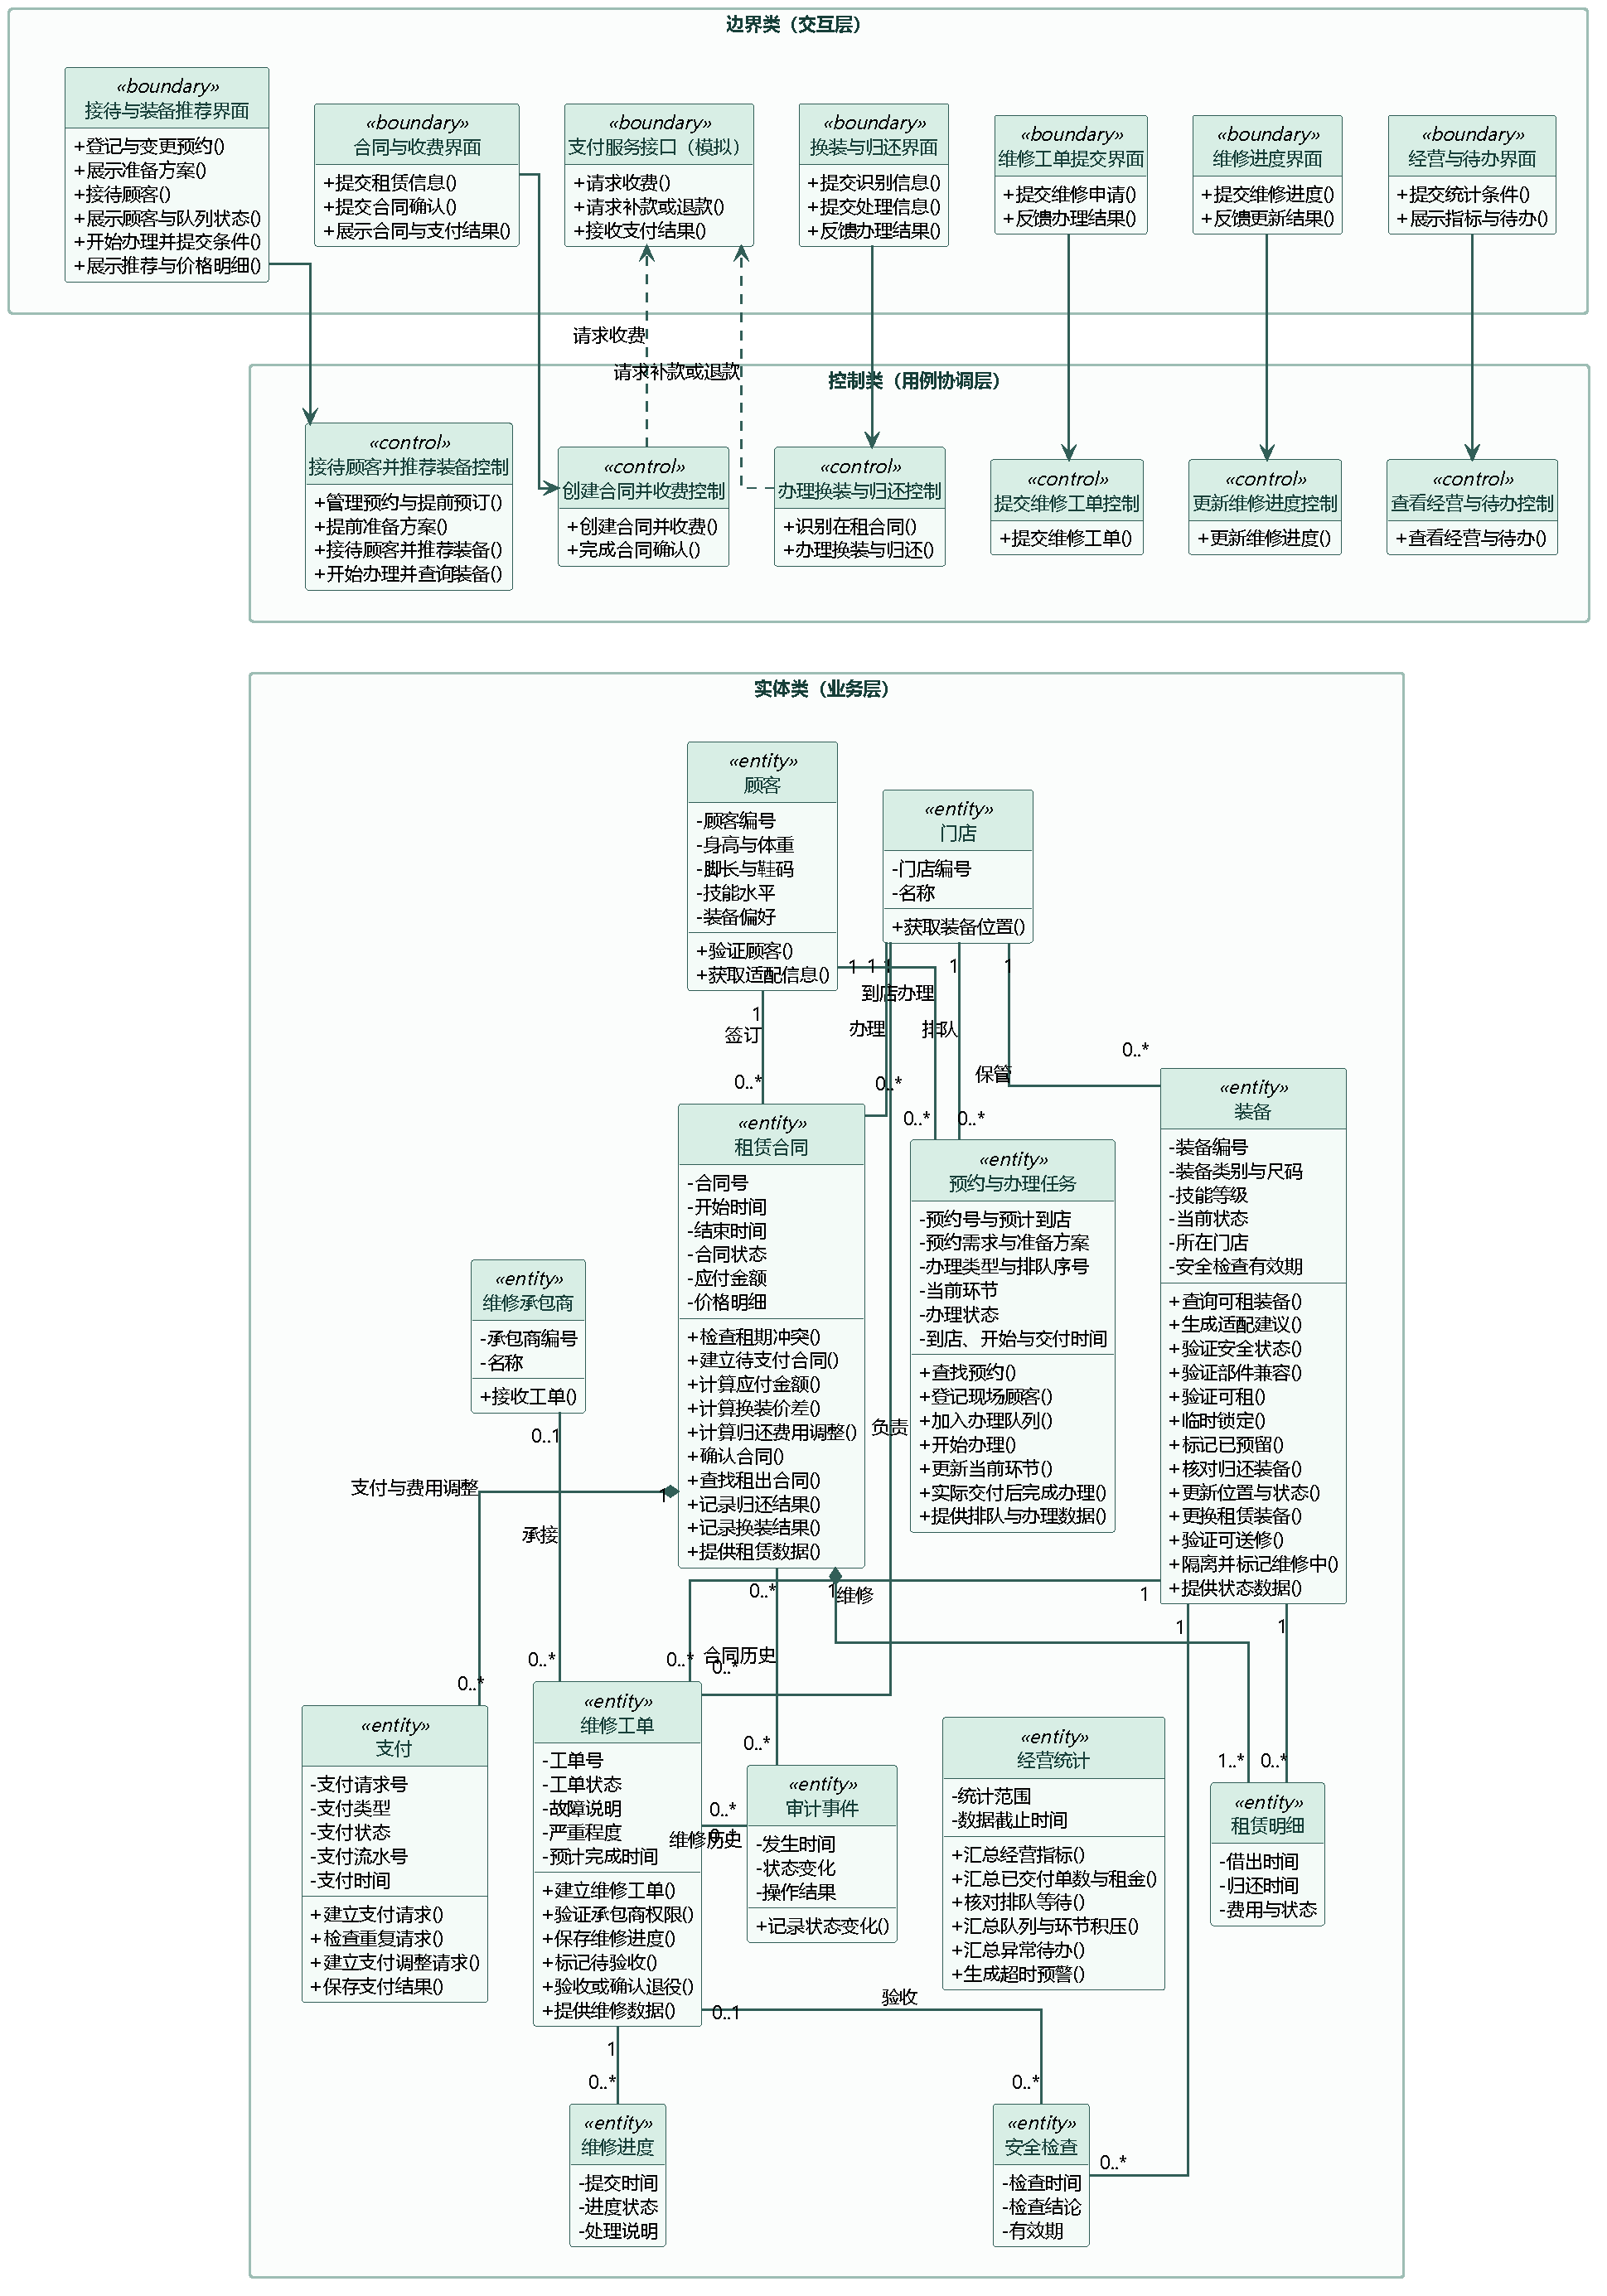
\includegraphics[width=\textwidth,height=0.79\textheight,keepaspectratio]{latex-assets/C1.pdf}
\captionof{figure}{BSR 分析类图}\label{fig:c1}
\end{minipage}\par\clearpage

\subsection{分析序列图}

每个系统用例对应一张分析序列图。

\singlepagediagram{latex-assets/C2_01.pdf}{UC01 接待顾客并推荐装备 - 分析序列图}{fig:c201}
\tallsequence{latex-assets/C2_02.pdf}{UC02 创建合同并收费 - 分析序列图}{fig:c202}
\tallsequence{latex-assets/C2_03.pdf}{UC03 办理换装与归还 - 分析序列图}{fig:c203}
\singlepagediagram{latex-assets/C2_04.pdf}{UC04 提交维修工单 - 分析序列图}{fig:c204}
\singlepagediagram{latex-assets/C2_05.pdf}{UC05 更新维修进度 - 分析序列图}{fig:c205}
\singlepagediagram{latex-assets/C2_06.pdf}{UC06 查看经营与待办 - 分析序列图}{fig:c206}

\clearpage
\subsection{分析状态机图}

状态图结合办理类型和持久化状态区分预订与现场接待；预订确认不等于实际到店，校验和保存作为转换条件。UC06 为只读查询，由分析序列图描述。

\singlepagediagram{latex-assets/C3_01.pdf}{UC01 接待顾客并推荐装备 - 预订与现场办理状态机图}{fig:c301}
\singlepagediagram{latex-assets/C3_02.pdf}{UC02 创建合同并收费 - 租赁合同状态机图}{fig:c302}
\singlepagediagram{latex-assets/C3_03.pdf}{UC03 办理换装与归还 - 租赁合同状态机图}{fig:c303}
\singlepagediagram{latex-assets/C3_04.pdf}{UC04 提交维修工单 - 维修工单状态机图}{fig:c304}
\singlepagediagram{latex-assets/C3_05.pdf}{UC05 更新维修进度 - 关联装备状态机图}{fig:c305}


\clearpage
\section{设计}

设计阶段把分析模型细化为数据、业务逻辑和表示层方案。三层保持单向依赖：表示层依赖业务逻辑层，业务逻辑层通过接口使用数据访问能力。

\subsection{数据访问层设计}

\subsubsection{数据库总 ERD}

本系统共设计 20 张物理表和 1 个经营统计视图。总 ERD（图 \ref{fig:d1}）标明主键、外键、表间基数和视图来源。完整业务字段及约束见分区 ERD 与数据表设计。

\singlepagediagram{latex-assets/D1.pdf}{BSR 数据库总 ERD}{fig:d1}

\clearpage
\subsubsection{分区 ERD}

\paragraph{客户与接待子模式}
\singlepagediagram{latex-assets/D2.pdf}{BSR 客户与接待子模式 ERD}{fig:d2}

\clearpage
\paragraph{装备与库存子模式}
\singlepagediagram{latex-assets/D3.pdf}{BSR 装备与库存子模式 ERD}{fig:d3}

\clearpage
\paragraph{租赁与支付子模式}
\singlepagediagram{latex-assets/D4.pdf}{BSR 租赁与支付子模式 ERD}{fig:d4}

\clearpage
\paragraph{维修、安全检查与审计子模式}
\singlepagediagram{latex-assets/D5.pdf}{BSR 维修、安全检查与审计子模式 ERD}{fig:d5}

\clearpage
\subsubsection{数据表设计}

\setcounter{table}{0}

\dbtable{顾客信息表（\texttt{customer}）}{tab:customer}{
\texttt{customer\_id} & 顾客编号 & BIGINT & PK，非空，自增\\
\texttt{phone} & 手机号码 & VARCHAR(30) & UQ，非空\\
\texttt{name} & 顾客姓名 & NVARCHAR(100) & 非空\\
\texttt{email} & 电子邮箱 & VARCHAR(255) & 可空\\
\texttt{created\_at} & 创建时间 & TIMESTAMP & 非空，默认当前时间\\}

\dbtable{顾客适配档案表（\texttt{customer\_fit\_profile}）}{tab:fitprofile}{
\texttt{profile\_id} & 档案编号 & BIGINT & PK，非空，自增\\
\texttt{customer\_id} & 顾客编号 & BIGINT & FK$\rightarrow$\texttt{customer}，UQ，非空\\
\texttt{height\_cm} & 身高（cm） & DECIMAL(5,2) & 可空\\
\texttt{weight\_kg} & 体重（kg） & DECIMAL(5,2) & 可空\\
\texttt{foot\_length\_mm} & 实测脚长（mm） & SMALLINT & 可空\\
\texttt{shoe\_size} & 日常鞋码（EU） & DECIMAL(4,1) & 可空，仅作参考\\
\texttt{skill\_level} & 滑雪技能等级 & VARCHAR(20) & 可空\\
\texttt{equipment\_preference} & 装备偏好 & NVARCHAR(255) & 可空\\
\texttt{updated\_at} & 最后更新时间 & TIMESTAMP & 非空，默认当前时间\\}

\dbtable{门店信息表（\texttt{store}）}{tab:store}{
\texttt{store\_id} & 门店编号 & BIGINT & PK，非空，自增\\
\texttt{store\_code} & 门店代码 & VARCHAR(20) & UQ，非空\\
\texttt{name} & 门店名称 & NVARCHAR(100) & 非空\\
\texttt{address} & 门店地址 & NVARCHAR(255) & 可空\\
\texttt{active} & 是否启用 & BOOLEAN & 非空，默认 true\\}

\dbtable{系统用户表（\texttt{user\_account}）}{tab:useraccount}{
\texttt{user\_id} & 用户编号 & BIGINT & PK，非空，自增\\
\texttt{username} & 登录账号 & VARCHAR(80) & UQ，非空\\
\texttt{store\_id} & 所属门店编号 & BIGINT & FK$\rightarrow$\texttt{store}，可空\\
\texttt{contractor\_id} & 所属维修承包商编号 & BIGINT & FK$\rightarrow$\texttt{repair\_contractor}，可空\\
\texttt{role\_type} & 用户角色 & VARCHAR(30) & 非空\\
\texttt{display\_name} & 显示姓名 & NVARCHAR(100) & 非空\\
\texttt{active} & 是否启用 & BOOLEAN & 非空，默认 true\\
\texttt{last\_login\_at} & 最后登录时间 & TIMESTAMP & 可空\\}

\dbtable{服务预约表（\texttt{service\_reservation}）}{tab:reservation}{
\texttt{reservation\_id} & 预约编号 & BIGINT & PK，非空，自增\\
\texttt{reservation\_no} & 预约单号 & VARCHAR(40) & UQ，非空\\
\texttt{customer\_id} & 顾客编号 & BIGINT & FK$\rightarrow$\texttt{customer}，非空\\
\texttt{store\_id} & 预约门店编号 & BIGINT & FK$\rightarrow$\texttt{store}，非空\\
\texttt{requested\_start\_at} & 租赁计划开始时间 & TIMESTAMP & 非空\\
\texttt{requested\_end\_at} & 租赁计划结束时间 & TIMESTAMP & 非空\\
\texttt{appointment\_at} & 预计到店时间 & TIMESTAMP & 新预约必填；旧记录可空\\
\texttt{requirements} & 本次需求快照 & JSON/TEXT & 身体参数、类别、接口、归还门店及备注；旧记录可空\\
\texttt{preparation} & 备选方案与联系记录 & JSON/TEXT & 可空；不占用库存，修改需求后清空\\
\texttt{version} & 并发版本 & INTEGER & 非空，默认0；更新时校验\\
\texttt{source\_type} & 预约来源 & VARCHAR(20) & 非空；电话、微信、当面；兼容旧来源\\
\texttt{status} & 预约状态 & VARCHAR(30) & 非空\\
\texttt{created\_at} & 创建时间 & TIMESTAMP & 非空，默认当前时间\\}

\dbtable{办理任务表（\texttt{service\_task}）}{tab:servicetask}{
\texttt{task\_id} & 办理任务编号 & BIGINT & PK，非空，自增\\
\texttt{reservation\_id} & 来源预约编号 & BIGINT & FK$\rightarrow$\texttt{service\_reservation}，可空\\
\texttt{customer\_id} & 顾客编号 & BIGINT & FK$\rightarrow$\texttt{customer}，非空\\
\texttt{store\_id} & 办理门店编号 & BIGINT & FK$\rightarrow$\texttt{store}，非空\\
\texttt{assigned\_user\_id} & 负责员工编号 & BIGINT & FK$\rightarrow$\texttt{user\_account}，可空\\
\texttt{task\_type} & 办理类型 & VARCHAR(20) & 非空，默认现场接待；或提前预订\\
\texttt{queue\_no} & 排队序号 & INTEGER & 非空；提前预订为0，实际到店后分配\\
\texttt{current\_stage} & 当前办理环节 & VARCHAR(30) & 非空\\
\texttt{status} & 办理状态 & VARCHAR(30) & 非空\\
\texttt{enqueued\_at} & 到店排队时间 & TIMESTAMP & 提前预订及旧记录可空\\
\texttt{recommendation\_revision} & 推荐版本 & INTEGER & 非空，默认0\\
\texttt{started\_at} & 开始办理时间 & TIMESTAMP & 非空\\
\texttt{finished\_at} & 完成时间 & TIMESTAMP & 可空\\}

\dbtable{装备类别表（\texttt{equipment\_category}）}{tab:category}{
\texttt{category\_id} & 类别编号 & BIGINT & PK，非空，自增\\
\texttt{category\_code} & 类别代码 & VARCHAR(30) & UQ，非空\\
\texttt{name} & 类别名称 & NVARCHAR(80) & 非空\\
\texttt{safety\_interval\_days} & 安全检查间隔天数 & INTEGER & 非空\\
\texttt{active} & 是否启用 & BOOLEAN & 非空，默认 true\\}

\dbtable{装备型号表（\texttt{equipment\_model}）}{tab:equipmentmodel}{
\texttt{model\_id} & 型号编号 & BIGINT & PK，非空，自增\\
\texttt{category\_id} & 装备类别编号 & BIGINT & FK$\rightarrow$\texttt{equipment\_category}，非空\\
\texttt{model\_code} & 型号代码 & VARCHAR(40) & UQ，非空\\
\texttt{brand} & 品牌 & NVARCHAR(80) & 非空\\
\texttt{model\_name} & 型号名称 & NVARCHAR(120) & 非空\\
\texttt{size\_spec} & 尺码或规格 & VARCHAR(30) & 非空\\
\texttt{skill\_level} & 适用技能等级 & VARCHAR(20) & 可空\\
\texttt{compatibility\_rule} & 部件兼容规则 & JSON/TEXT & 可空\\}

\dbtable{单件装备表（\texttt{equipment}）}{tab:equipment}{
\texttt{equipment\_id} & 装备编号 & BIGINT & PK，非空，自增\\
\texttt{asset\_no} & 资产编号 & VARCHAR(40) & UQ，非空；品类--尺寸--两位序号\\
\texttt{legacy\_asset\_no} & 原资产编号 & VARCHAR(40) & 可空；保留旧编号检索\\
\texttt{model\_id} & 装备型号编号 & BIGINT & FK$\rightarrow$\texttt{equipment\_model}，非空\\
\texttt{current\_store\_id} & 当前所在门店编号 & BIGINT & FK$\rightarrow$\texttt{store}，非空\\
\texttt{status} & 装备状态 & VARCHAR(30) & 非空\\
\texttt{acquired\_at} & 入库日期 & DATE & 非空\\
\texttt{retired\_at} & 退役日期 & DATE & 可空\\
\texttt{version} & 并发版本号 & INTEGER & 非空，默认 0\\}

\dbtable{装备位置历史表（\texttt{equipment\_location\_history}）}{tab:locationhistory}{
\texttt{movement\_id} & 位置变更编号 & BIGINT & PK，非空，自增\\
\texttt{equipment\_id} & 装备编号 & BIGINT & FK$\rightarrow$\texttt{equipment}，非空\\
\texttt{from\_store\_id} & 原门店编号 & BIGINT & FK$\rightarrow$\texttt{store}，可空\\
\texttt{to\_store\_id} & 目标门店编号 & BIGINT & FK$\rightarrow$\texttt{store}，非空\\
\texttt{contract\_id} & 相关合同编号 & BIGINT & FK$\rightarrow$\texttt{rental\_contract}，可空\\
\texttt{recorded\_by\_user\_id} & 记录人编号 & BIGINT & FK$\rightarrow$\texttt{user\_account}，非空\\
\texttt{movement\_type} & 位置变更类型 & VARCHAR(30) & 非空\\
\texttt{moved\_at} & 变更时间 & TIMESTAMP & 非空\\
\texttt{note} & 变更说明 & NVARCHAR(255) & 可空\\}

\dbtable{租赁合同表（\texttt{rental\_contract}）}{tab:contract}{
\texttt{contract\_id} & 合同编号 & BIGINT & PK，非空，自增\\
\texttt{contract\_no} & 合同单号 & VARCHAR(40) & UQ，非空\\
\texttt{service\_task\_id} & 来源办理任务编号 & BIGINT & FK$\rightarrow$\texttt{service\_task}，UQ，非空\\
\texttt{customer\_id} & 顾客编号 & BIGINT & FK$\rightarrow$\texttt{customer}，非空\\
\texttt{pickup\_store\_id} & 取件门店编号 & BIGINT & FK$\rightarrow$\texttt{store}，非空\\
\texttt{return\_store\_id} & 实际归还门店编号 & BIGINT & FK$\rightarrow$\texttt{store}，可空\\
\texttt{start\_at} & 租赁开始时间 & TIMESTAMP & 非空\\
\texttt{end\_at} & 计划结束时间 & TIMESTAMP & 非空\\
\texttt{status} & 合同状态 & VARCHAR(30) & 非空\\
\texttt{amount\_due} & 应付金额 & DECIMAL(12,2) & 非空，默认 0\\
\texttt{price\_snapshot} & 价格规则快照 & JSON/TEXT & 非空\\
\texttt{version} & 并发版本号 & INTEGER & 非空，默认 0\\}

\dbtable{合同装备明细表（\texttt{rental\_item}）}{tab:rentalitem}{
\texttt{rental\_item\_id} & 租赁明细编号 & BIGINT & PK，非空，自增\\
\texttt{contract\_id} & 合同编号 & BIGINT & FK$\rightarrow$\texttt{rental\_contract}，非空，联合唯一\\
\texttt{equipment\_id} & 装备编号 & BIGINT & FK$\rightarrow$\texttt{equipment}，非空，联合唯一\\
\texttt{replaces\_item\_id} & 被替换明细编号 & BIGINT & FK$\rightarrow$\texttt{rental\_item}，可空\\
\texttt{rented\_from} & 实际租用开始时间 & TIMESTAMP & 非空，联合唯一\\
\texttt{rented\_to} & 实际租用结束时间 & TIMESTAMP & 可空\\
\texttt{quoted\_price} & 明细报价 & DECIMAL(12,2) & 非空\\
\texttt{item\_status} & 明细状态 & VARCHAR(30) & 非空\\}

\dbtable{支付请求表（\texttt{payment\_request}）}{tab:paymentrequest}{
\texttt{payment\_request\_id} & 支付请求编号 & BIGINT & PK，非空，自增\\
\texttt{request\_no} & 业务请求号 & VARCHAR(64) & UQ，非空\\
\texttt{contract\_id} & 合同编号 & BIGINT & FK$\rightarrow$\texttt{rental\_contract}，非空\\
\texttt{request\_type} & 请求类型 & VARCHAR(20) & 非空\\
\texttt{amount} & 请求金额 & DECIMAL(12,2) & 非空\\
\texttt{status} & 请求状态 & VARCHAR(30) & 非空\\
\texttt{created\_at} & 创建时间 & TIMESTAMP & 非空，默认当前时间\\}

\dbtable{支付流水表（\texttt{payment\_transaction}）}{tab:paymenttransaction}{
\texttt{transaction\_id} & 支付流水编号 & BIGINT & PK，非空，自增\\
\texttt{payment\_request\_id} & 支付请求编号 & BIGINT & FK$\rightarrow$\texttt{payment\_request}，非空，联合唯一\\
\texttt{provider\_transaction\_no} & 第三方流水号 & VARCHAR(80) & UQ，可空\\
\texttt{attempt\_no} & 请求尝试次数 & INTEGER & 非空，联合唯一\\
\texttt{amount} & 实际处理金额 & DECIMAL(12,2) & 非空\\
\texttt{status} & 流水状态 & VARCHAR(30) & 非空\\
\texttt{response\_code} & 第三方响应代码 & VARCHAR(40) & 可空\\
\texttt{processed\_at} & 处理完成时间 & TIMESTAMP & 可空\\}

\dbtable{维修承包商表（\texttt{repair\_contractor}）}{tab:contractor}{
\texttt{contractor\_id} & 承包商编号 & BIGINT & PK，非空，自增\\
\texttt{contractor\_code} & 承包商代码 & VARCHAR(30) & UQ，非空\\
\texttt{name} & 承包商名称 & NVARCHAR(120) & 非空\\
\texttt{contact\_phone} & 联系电话 & VARCHAR(30) & 非空\\
\texttt{active} & 是否启用 & BOOLEAN & 非空，默认 true\\}

\dbtable{维修工单表（\texttt{repair\_order}）}{tab:repairorder}{
\texttt{repair\_order\_id} & 维修工单编号 & BIGINT & PK，非空，自增\\
\texttt{ticket\_no} & 工单号 & VARCHAR(40) & UQ，非空\\
\texttt{equipment\_id} & 故障装备编号 & BIGINT & FK$\rightarrow$\texttt{equipment}，非空\\
\texttt{contractor\_id} & 维修承包商编号 & BIGINT & FK$\rightarrow$\texttt{repair\_contractor}，可空\\
\texttt{created\_by\_user\_id} & 建立人编号 & BIGINT & FK$\rightarrow$\texttt{user\_account}，非空\\
\texttt{status} & 工单状态 & VARCHAR(30) & 非空\\
\texttt{fault\_description} & 故障描述 & NVARCHAR(500) & 非空\\
\texttt{responsible\_store\_id} & 责任门店 & INTEGER & FK$\rightarrow$\texttt{store}，旧记录可空\\
\texttt{severity} & 严重程度 & TEXT & 低、中、高，旧记录可空\\
\texttt{estimated\_completion\_at} & 预计完成时间 & TIMESTAMP & 未接单或旧记录可空\\
\texttt{opened\_at} & 建立时间 & TIMESTAMP & 非空\\
\texttt{completed\_at} & 完成时间 & TIMESTAMP & 可空\\
\texttt{version} & 并发版本号 & INTEGER & 非空，默认 0\\}

\dbtable{维修进度表（\texttt{repair\_update}）}{tab:repairupdate}{
\texttt{repair\_update\_id} & 维修进度编号 & BIGINT & PK，非空，自增\\
\texttt{repair\_order\_id} & 维修工单编号 & BIGINT & FK$\rightarrow$\texttt{repair\_order}，非空\\
\texttt{submitted\_by\_user\_id} & 提交人编号 & BIGINT & FK$\rightarrow$\texttt{user\_account}，非空\\
\texttt{progress\_status} & 维修进度状态 & VARCHAR(30) & 非空\\
\texttt{note} & 进度说明 & NVARCHAR(500) & 非空\\
\texttt{created\_at} & 提交时间 & TIMESTAMP & 非空，默认当前时间\\}

\dbtable{安全检查表（\texttt{safety\_inspection}）}{tab:safetyinspection}{
\texttt{inspection\_id} & 检查记录编号 & BIGINT & PK，非空，自增\\
\texttt{equipment\_id} & 装备编号 & BIGINT & FK$\rightarrow$\texttt{equipment}，非空\\
\texttt{repair\_order\_id} & 相关维修工单编号 & BIGINT & FK$\rightarrow$\texttt{repair\_order}，可空\\
\texttt{inspector\_user\_id} & 检查人编号 & BIGINT & FK$\rightarrow$\texttt{user\_account}，非空\\
\texttt{result} & 检查结果 & VARCHAR(30) & 非空\\
\texttt{inspected\_at} & 检查时间 & TIMESTAMP & 非空\\
\texttt{valid\_until} & 检查有效期 & DATE & 可空\\
\texttt{note} & 检查说明 & NVARCHAR(500) & 可空\\}

\dbtable{审计事件表（\texttt{audit\_event}）}{tab:auditevent}{
\texttt{audit\_event\_id} & 审计事件编号 & BIGINT & PK，非空，自增\\
\texttt{actor\_user\_id} & 操作用户编号 & BIGINT & FK$\rightarrow$\texttt{user\_account}，可空\\
\texttt{event\_type} & 事件类型 & VARCHAR(40) & 非空\\
\texttt{from\_status} & 变更前状态 & VARCHAR(30) & 可空\\
\texttt{to\_status} & 变更后状态 & VARCHAR(30) & 可空\\
\texttt{result} & 操作结果 & VARCHAR(30) & 非空\\
\texttt{event\_store\_id} & 事件发生门店 & INTEGER & FK$\rightarrow$\texttt{store}，可空\\
\texttt{occurred\_at} & 发生时间 & TIMESTAMP & 非空，默认当前时间\\}

\dbtable{审计对象表（\texttt{audit\_event\_target}）}{tab:audittarget}{
\texttt{audit\_target\_id} & 审计对象编号 & BIGINT & PK，非空，自增\\
\texttt{audit\_event\_id} & 审计事件编号 & BIGINT & FK$\rightarrow$\texttt{audit\_event}，非空，联合唯一\\
\texttt{entity\_type} & 业务对象类型 & VARCHAR(40) & 非空，联合唯一\\
\texttt{entity\_id} & 业务对象主键值 & BIGINT & 非空，联合唯一\\}

\dbtable{经营统计视图（\texttt{vw\_operating\_metric}）}{tab:metricview}{
\texttt{metric\_date} & 指标日期 & DATE & 只读视图字段\\
\texttt{store\_id} & 门店编号 & BIGINT & 来源于 \texttt{store.store\_id}\\
\texttt{metric\_code} & 指标代码 & VARCHAR(40) & 只读视图字段\\
\texttt{metric\_value} & 指标数值 & DECIMAL(14,2) & 只读视图字段\\
\texttt{calculated\_at} & 指标计算时间 & TIMESTAMP & 只读视图字段\\}

\clearpage
\subsection{业务逻辑层设计}

业务逻辑层采用分层设计，把用例协调、业务规则和数据持久化职责分开。本节说明职责边界、聚合与服务，不涉及代码实现；表示层不得直接修改数据库，所有状态变化均需经由应用服务和领域规则校验。

{\small
\begin{longtable}{L{2.6cm}L{4.5cm}L{8.2cm}}
\toprule
\tablehead{层次} & \tablehead{承担的职责} & \tablehead{设计安排}\\
\midrule
\endfirsthead
\toprule
\tablehead{层次} & \tablehead{承担的职责} & \tablehead{设计安排}\\
\midrule
\endhead
表示层 & 接收输入、展示结果并完成格式校验。 & 对应六个系统用例设置操作入口，只提交命令和查询，不承载计价、适配或状态判断规则。\\
应用层 & 按用例组织步骤、控制事务并协调领域对象。 & 分别设计接待推荐、合同收费、换装归还、维修提交、维修更新和经营查询六类应用服务。\\
领域层 & 保存核心业务对象及其状态规则。 & 围绕租赁合同、装备、维修工单和办理任务划分聚合，并设计适配推荐、费用计算、支付防重和经营汇总服务。\\
基础设施层 & 为上层提供数据持久化、支付接口、审计和定时任务能力。 & 通过仓储接口与外部服务适配接口隔离数据库和第三方支付服务，线上读取私有云存储中的 SQLite 快照，事务后按版本条件保存；本地使用 SQLite，支付使用模拟适配器。\\
\bottomrule
\end{longtable}}

业务逻辑设计需要保证四类核心约束：同一装备在同一租期不得进入两份有效合同；检查过期、维修中或待验收装备不得出租；同一支付请求不得重复收费或退款；每次关键状态变化均形成审计事件。跨对象规则集中在领域服务中，避免由界面操作人员自行判断。

\subsection{课程演示业务规则}
租期按24小时为一天，不足一天按一天计。双板、雪靴、雪杖、头盔的基础日租金分别为110、65、20、30元，押金分别为180、100、30、50元；技能档位每升一级，日租金加25元。换装按剩余租期结算租金和押金差额；归还时结算逾期及损坏费用，提前归还不重算约定租金。

预约登记不占库存，完成模拟付款后才按租期预留装备。预计到店时间用于备货，不限制预约人数，也不保证免排队。实际到店统一排队；付款取件后可试装，不合适按原合同换装，预订取件不重复收费。

付款临时占用最长15分钟，超时释放本次占用；取消已付款合同须模拟退款。出租前校验租期、适配、接口及安全状态；临近尺寸须试穿核对，维修、退役或检查无效的装备不得出租。跨店归还更新实际位置。

双板和雪杖长度用cm，雪靴适配脚长用mm，头盔用XS至XL；日常鞋码仅供参考。装备名称和品类编号保持统一。

\clearpage
\subsection{表示层设计}

表示层围绕六个系统用例设计六个功能区。

{\small
\begin{longtable}{L{3.5cm}L{3.5cm}L{8.3cm}}
\toprule
\tablehead{界面} & \tablehead{对应功能区} & \tablehead{主要信息与交互要求}\\
\midrule
\endfirsthead
\toprule
\tablehead{界面} & \tablehead{对应功能区} & \tablehead{主要信息与交互要求}\\
\midrule
\endhead
接待与装备推荐界面 & 接待管理 & 分为预约安排、预约准备、到店办理。提前选装、核对合同并模拟付款后预留装备；到店后按顺序核对取件。现场顾客到店选装收费。队列统一展示排队与办理记录，显示当前状态、合同及取件信息；取件后可试装换装，可记录离店未办理。\\
合同与收费界面 & 合同办理 & 在确认前完整展示装备明细、租期、价格和规则；清楚区分待支付、处理中、成功与失败状态。\\
换装与归还界面 & 归还与换装 & 在同一入口选择业务类型，记录检查结果、实际归还门店、替换装备和补退款结果，分别展示合同与费用状态。\\
维修工单提交界面 & 维修登记 & 显示装备当前状态和已有工单，采集故障现象、严重程度、责任门店及承包商。\\
维修进度界面 & 维修跟踪 & 按工单状态和责任门店筛选，显示预计完成时间及进度；责任门店验收或确认退役。\\
经营与待办界面 & 经营概览 & 分设当前概览、经营统计、审计记录；经营统计保留四项主指标，待核对记录简要提示并可展开，其他业务数量折叠为紧凑数据格；展示两店对比与分类待办。审计关联对象使用中文名称和业务编号，可检索并只读查看详情，原事件保留。\\
\bottomrule
\end{longtable}}

所有界面统一采用绿色为主的低干扰视觉基调，并遵守三项交互约束：同一业务对象只保留一个主要修改入口；提交前展示将发生的状态变化；失败时返回可理解的原因和可继续执行的操作。

\end{document}
